% =====================================================================
%  monoT5 Encoder Per-Head Activation Patching + Ablation — Report
%  Compile with:  pdflatex encoder_head_patching_experiment_report.tex  (run twice)
%  Figure paths are relative to this file (outputs/...), so compile
%  from the 11_monot5_encoder_head_patching/ directory.
% =====================================================================
\documentclass[11pt]{article}

\usepackage[margin=1in]{geometry}
\usepackage{amsmath, amssymb}
\usepackage{graphicx}
\usepackage{booktabs}
\usepackage{longtable}
\usepackage{array}
\usepackage{float}
\usepackage{xcolor}
\usepackage{caption}
\usepackage{enumitem}
\usepackage{listings}
\usepackage[hidelinks]{hyperref}

\definecolor{codegray}{gray}{0.95}
\lstset{
  basicstyle=\ttfamily\footnotesize,
  backgroundcolor=\color{codegray},
  breaklines=true,
  frame=single,
  columns=fullflexible,
  keepspaces=true,
}

\newcommand{\fwd}{\ensuremath{e^{\mathrm{fwd}}}}
\newcommand{\rev}{\ensuremath{e^{\mathrm{rev}}}}
\newcommand{\score}{\operatorname{score}}
\newcommand{\comb}{\ensuremath{e^{\mathrm{comb}}}}

\title{\textbf{Per-Head Activation Patching and Ablation of the monoT5 \\[2pt]
Encoder under Keyword-Stuffing Adversarial Attacks} \\[6pt]
\large The Encoder-Side Analog of the Decoder Head-Localisation Study}
\author{Information-Retrieval Adversarial-Evaluation Project}
\date{\today}

\begin{document}
\maketitle

\begin{abstract}
Per-head causal patching of all 144 monoT5 encoder self-attention head-slots
(canonical attack, $n{=}100$, plus the full 105-attack grid, $n{=}10$/attack) finds the
layer-9--11 effect \textbf{sparse, not uniform}: 18 of 144 head-slots exceed the
project-wide 0.02 flag threshold, with the top 5 (\texttt{L11H3}, \texttt{L11H4},
\texttt{L10H6}, \texttt{L10H2}, \texttt{L10H4}) robust on 100--104 of 105 attacks. Summing
flagged heads' individual peak effects gives $0.85$ against $0.48$ for the existing
whole-layer effect (Experiment 6) — a $1.76\times$, \textbf{super-additive} result that
directly \emph{contradicts} the sub-additive pattern predicted from Experiment 6's
template-position finding (stated before computing). Cross-referencing against the
layer-9 document$\to$query attention-mass anomaly shows only 6 of 48 causally-important
(layer, head) cells at layers 8--11 actually carry elevated attention mass alongside their
causal effect; the majority of layer-10--11 heads are causally important with
\emph{unremarkable} raw attention — the mechanism is not visible in the attention
matrix for most of the effect. The attack-token-as-hub hypothesis holds on average
(flagged heads' mean query-directed elevation $+0.14$ vs.\ unflagged heads' $+0.11$) but
not uniformly: the single strongest head (\texttt{L9H6}) shows the attack token attending
\emph{less} to the query than a random document token, while another (\texttt{L9H3})
shows the largest positive elevation measured — at least two distinct mechanisms
contribute to the same layer-9--11 effect. Zero ablation is confirmed to grossly
over-attribute importance relative to mean/control ablation (Experiment 3's decoder
finding transfers unchanged to the encoder).
\end{abstract}

\tableofcontents
\newpage

% =====================================================================
\section{Introduction and Motivation}
% =====================================================================

Experiments 1 and 6 localised the keyword-stuffing attack's causal effect and the
document$\to$query contamination effect to \emph{whole} encoder self-attention layers
9--11 (all 12 heads patched together). Experiment 3 asked the equivalent
head-granularity question on the decoder and found the effect sparse: only 33 of 288
decoder head-slots mattered. This leaves the same gap on the encoder side, explicitly
deferred as out-of-scope in both Experiment 3's and Experiment 6's Limitations sections:
is the encoder's layer-9--11 effect spread evenly across all 12 heads per layer, or
concentrated in a sparse subset? A reviewer familiar with Experiment 3 would ask why head
decomposition stopped at the decoder; this experiment closes that gap, and additionally
cross-references the result against two descriptive findings Experiment 6 could not
explain at head granularity: a layer-9 document$\to$query attention-mass anomaly, and
whether the attack token itself acts as an active aggregator of query context.

% =====================================================================
\section{Background}
% =====================================================================

\subsection{Where a ``head'' lives in T5 attention}

T5Attention computes, per position:
\begin{equation}
\text{inner} = \text{concat}(h_0, \dots, h_{11}) \in \mathbb{R}^{12 \cdot d_{kv}}, \qquad
\text{out} = W_o \cdot \text{inner} \in \mathbb{R}^{d_{model}}
\label{eq:headconcat}
\end{equation}
Head $h$ occupies the contiguous slice $[h \cdot d_{kv} : (h{+}1) \cdot d_{kv}]$ of
\text{inner}. $W_o$ has no bias, so replacing or zeroing head $h$'s slice replaces or
zeroes exactly that head's additive contribution to the residual stream — the same
mechanism Experiment 3 uses for the decoder, applied here to
\texttt{encoder.block[layer].layer[0].SelfAttention.o}.

\subsection{Scope: encoder-only, one component, 144 head-slots}

The encoder has exactly one attention sublayer per block (\texttt{layer[0]}; \texttt{
layer[1]} is the feed-forward, no heads), so scope is $(layer, head)$ only:
12 layers $\times$ 12 heads $=$ \textbf{144 head-slots}, versus Experiment 3's
$2 \times 12 \times 12 = 288$. All patching is \textbf{whole-sequence} (every position at
once), matching Experiment 6's whole-block conditions' granularity, not its per-position
template-token patching — a joint head$\times$position sweep is out of scope this pass.

\subsection{Why the decoder's exactness-preserving speedup only half-applies}

Experiment 3 gets two speedups: encoder-output reuse (decoder-only patches never need the
encoder to re-execute) and batched-over-heads decoder passes (score all 12 heads of one
slot in a single batch-12 decoder pass). Encoder self-attention patches happen
\emph{inside} the encoder's own forward computation, so encoder-output reuse does not
apply — every (layer, direction) unit re-executes the encoder (the same limitation
Experiment 6's whole-block encoder patching has). The batched-over-heads trick still
applies, translated: one batched (batch$=12$) encoder-then-decoder pass, where row $h$ has
only head $h$'s \texttt{.o}-input slice patched, scores all 12 heads of a layer at once —
measured directly at $\approx$1--2~s/example for all 144 head-slots $\times$ 2 ablation
methods, comparable to Experiment 6's per-example cost.

\subsection{Scoring and effect formulas (unchanged from Experiment 1)}

$\score = \text{logit}(\text{true}) - \text{logit}(\text{false})$ at the single decoder
step. For head $h$ at layer $L$:
\begin{align}
\fwd_{L,h} &= \frac{\score(\text{control}, \text{head } h \to \text{attack activation}) - \score_{\text{control}}}{\Delta} \label{eq:hfwd}\\
\rev_{L,h} &= \frac{\score_{\text{attack}} - \score(\text{attack}, \text{head } h \to \text{control activation})}{\Delta} \label{eq:hrev}\\
\comb_{L,h} &= \min(\fwd_{L,h}, \rev_{L,h}) \label{eq:hcomb}
\end{align}
where $\Delta = \score_{\text{attack}} - \score_{\text{control}}$. \textbf{Mean/control}
ablation is the same computation as $\rev_{L,h}$'s replacement on the attack base
(\texttt{score\_ablated\_mean == score\_patched\_rev} by construction, computed once);
\textbf{zero} ablation sets the head's contribution to the zero vector. Mean/control
ablation is primary throughout (Experiment 3 established zero over-attributes
importance); zero is reported only for the Step~1 zero-vs-mean scatter.

% =====================================================================
\section{Methodology}
% =====================================================================

\subsection{Step 1 — Canonical attack, all 144 head-slots}
Attack \texttt{relevant\_start\_5}, $n{=}100$, all 12 layers $\times$ 12 heads, both
ablation methods. Layers processed in priority order 9, 10, 11, 8, \dots, 0 (an output
ordering only — every layer runs and is written).

\subsection{Step 2 — Full 105-attack sweep}
Same patch, $n{=}10$/attack, all 144 head-slots, not pre-filtered by the canonical
result. Heads flagged at combined\_effect $> 0.02$ (Experiment 6's template-position
threshold, for project-wide consistency).

\subsection{Step 3 — Additivity check}
\emph{Prediction stated before computing}: sub-additive, matching Experiment 6's
template-position finding (individual positions summed to $0.44\times$ the whole-span
effect). Sum of flagged heads' individual peak $\comb$ (layers 9--11, canonical) versus
the existing whole-layer \texttt{both} (query$\cup$document) effect at the same layers
(Experiment 6, read-only).

\subsection{Step 4 — Layer 8--11 per-head attention cross-reference}
Experiment 6's \texttt{normalized\_attention\_masses} averages over heads before any row
is written to disk — verified directly: \texttt{outputs/canonical/aggregated/
attention\_summary.csv} has no head column. No per-head attention tensor from
Experiment 6 survives to re-slice; this step recomputes attention fresh, on the
\emph{same} canonical-attack example set Step 1 used, clean vs.\ attacked input (matching
Experiment 6 Part 1's own convention, not the padded control).
2$\times$2 classification: mass ``high'' $>1.0\times$ uniform baseline; causal ``high''
$>0.02$.

\subsection{Step 5 — Attack-token-as-hub}
For heads flagged in Step 1 (canonical, layers 9--11): the attack token's own outgoing
attention to the query span and document span, versus a matched-count random
non-attack-document-token control (deterministic seed per example). Two falsifiable
predictions stated before running:
\begin{description}[leftmargin=1.4em,style=nextline]
  \item[Hub hypothesis] attack-token$\to$query mass is elevated over the random-token
  control, concentrated in the causally-flagged heads.
  \item[Passive hypothesis] no elevation, or elevation not concentrated in the flagged
  heads — contamination happens through some other pathway (e.g.\ broad residual-stream
  mixing), not the attack token's own attention pattern.
\end{description}

% =====================================================================
\section{Experimental Setup}
% =====================================================================

\begin{table}[H]
\centering
\caption{Configuration and scope.}
\begin{tabular}{ll}
\toprule
Parameter & Value \\
\midrule
Model checkpoint & \texttt{castorini/monot5-base-msmarco} \\
Scope & 12 encoder layers $\times$ 12 heads $=$ 144 head-slots, whole-sequence \\
Ablation methods & zero (secondary), mean/control (primary) \\
Canonical run & \texttt{relevant\_start\_5} $\times$ 100 examples \\
Full sweep & 105 attacks $\times$ 10 examples \\
Flag threshold & combined\_effect $> 0.02$ \\
Mass baseline & normalized\_mass $> 1.0\times$ uniform \\
\bottomrule
\end{tabular}
\end{table}

\noindent SLURM job on 1$\times$ L40 GPU, $\approx$20~minutes wall-clock for the full
pipeline (Steps 1--5 + aggregation): canonical run 100/100 examples used, zero alignment
failures ($\approx$1.3--2.6~s/example, 144 head-slots $\times$ 2 ablation methods); full
sweep 105/105 attacks $\times$ 10/10 examples, zero alignment failures
($\approx$0.9~s/example, 151{,}200 rows); Steps 4/5 100/100 examples each, zero alignment
failures.

% =====================================================================
\section{Results}
\label{sec:results}
% =====================================================================

\subsection{Localisation: the layer-9--11 effect is sparse, not uniform}
\label{sec:localisation}

\begin{figure}[H]
  \centering
  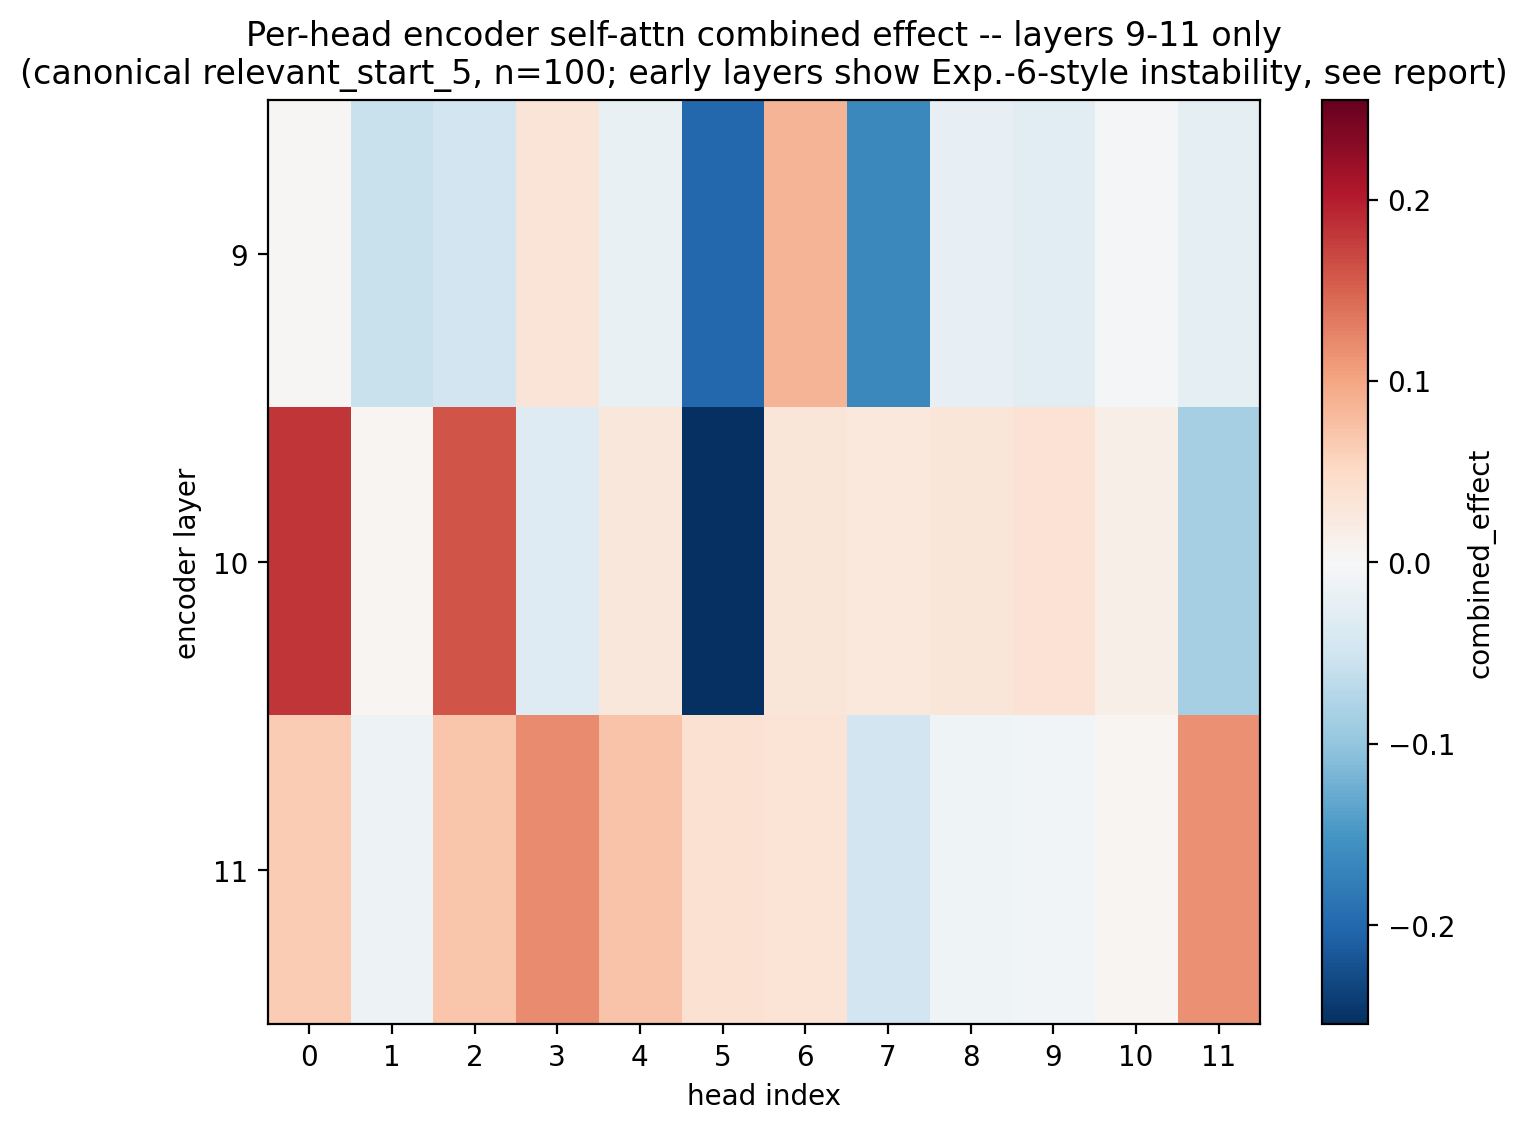
\includegraphics[width=0.7\textwidth]{outputs/plots/exp11_head_heatmap_canonical_late_layers.png}
  \caption{Per-head combined\_effect, layers 9--11 only (canonical attack, $n{=}100$).
  Early layers (0--8, not shown here — see Figure~\ref{fig:fullheatmap}) show large,
  sign-flipped outliers from the same residual-stream-incoherence mechanism
  Section~\ref{sec:earlylayerinstability} discusses, which would otherwise dominate the
  colour scale.}
  \label{fig:heatmaplate}
\end{figure}

\begin{table}[H]
\centering
\caption{Top 10 head-slots by mean combined\_effect (canonical attack, $n{=}100$).}
\label{tab:top10}
\begin{tabular}{lrrrrr}
\toprule
Head & $\fwd$ & $\rev$ & $\comb$ & drop(zero) & drop(mean) \\
\midrule
L10H0  & 0.200 & 0.222 & 0.182 & 0.116  & 0.302 \\
L10H2  & 0.172 & 0.276 & 0.161 & $-$0.739 & 0.364 \\
L11H3  & 0.127 & 0.165 & 0.121 & $-$0.266 & 0.232 \\
L11H11 & 0.132 & 0.149 & 0.117 & $-$0.098 & 0.190 \\
L9H6   & 0.218 & 0.242 & 0.087 & $-$2.178 & 0.326 \\
L11H4  & 0.085 & 0.140 & 0.073 & $-$0.987 & 0.222 \\
L11H2  & 0.080 & 0.090 & 0.072 & $-$0.563 & 0.134 \\
L11H0  & 0.067 & 0.140 & 0.065 & 0.119  & 0.203 \\
L8H11  & 0.060 & 0.174 & 0.057 & 0.009  & 0.238 \\
L11H5  & 0.049 & 0.080 & 0.039 & $-$0.071 & 0.118 \\
\bottomrule
\end{tabular}
\end{table}

Of 144 head-slots, \textbf{18} exceed the 0.02 flag threshold on the canonical attack.
Unlike Experiment 3's decoder result (33/288, concentrated almost entirely in
cross-attention), the encoder's important heads are spread across layers 8--11 with no
single layer dominating, and \texttt{L10H0}/\texttt{L10H2} — not a layer-11 head — carry
the single largest individual effects.

\subsection{Robustness across the full 105-attack grid}

Full-sweep flagging (peak combined\_effect $>0.02$, layers 9--11, pooled per head index)
confirms this is not a canonical-attack artefact: \texttt{L11H3} and \texttt{L11H4} exceed
threshold on \textbf{104 of 105} attacks, \texttt{L10H6} on 103/105, \texttt{L10H2} on
102/105, \texttt{L10H4} on 100/105 (Figure~\ref{fig:boxplot}) — as robust a signal as this
project has produced for any single-slot causal claim.

\begin{figure}[H]
  \centering
  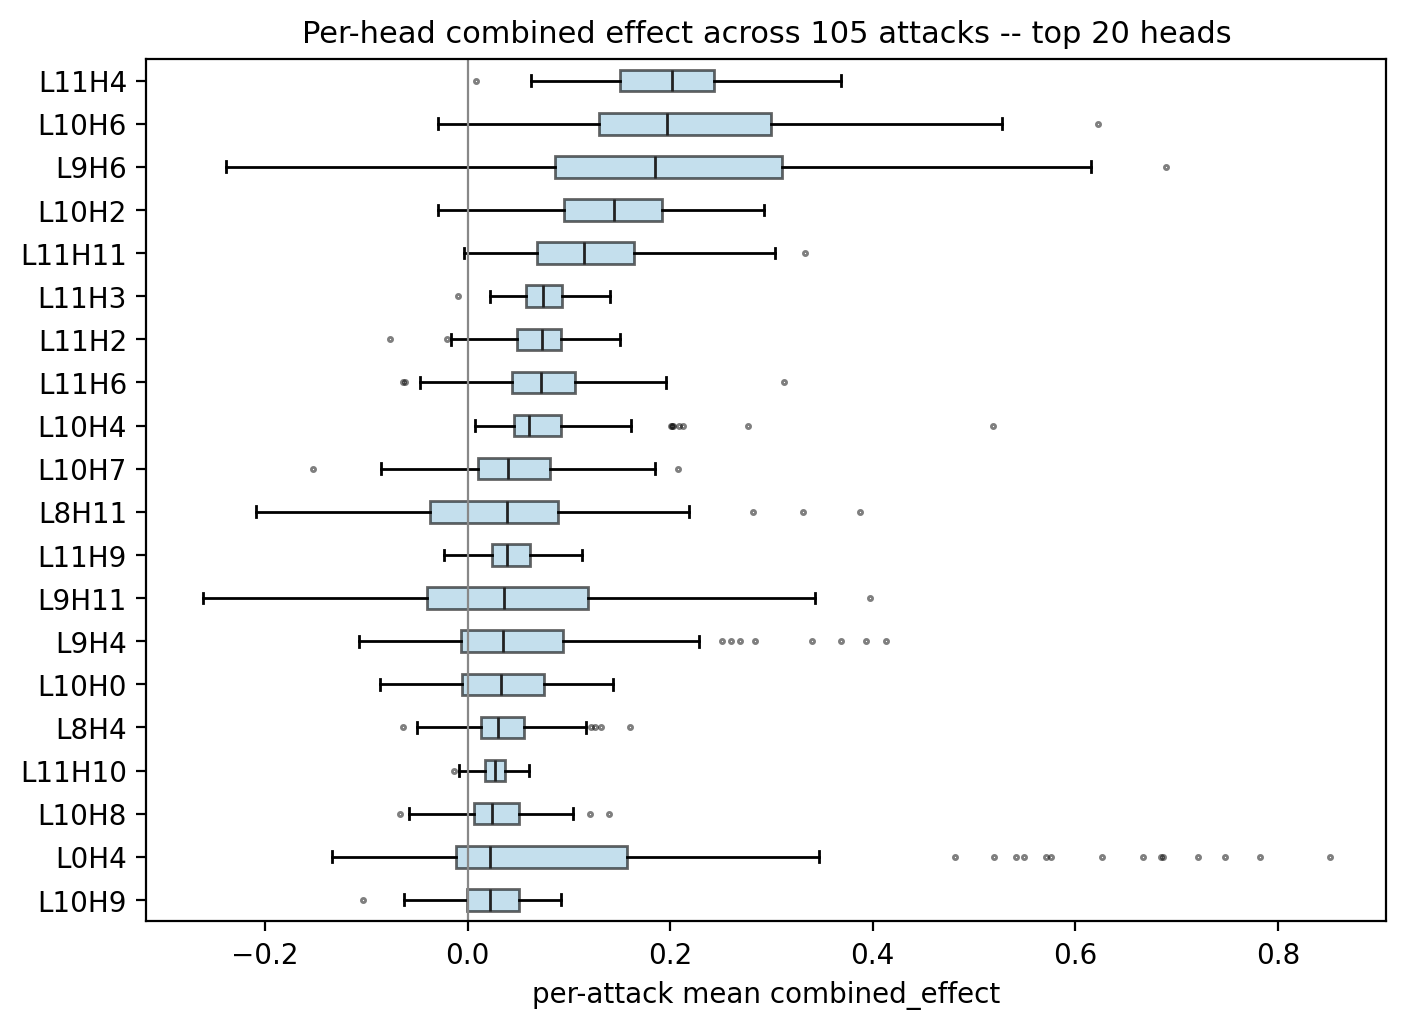
\includegraphics[width=0.75\textwidth]{outputs/plots/exp11_per_head_effect_across_attacks.png}
  \caption{Per-head combined\_effect distribution across all 105 attacks, top 20 heads by
  median. Tight boxes well above 0 (\texttt{L11H4}, \texttt{L10H2}, \texttt{L11H3}) are
  universal attack heads; \texttt{L0H4}'s wide scatter of high outliers (bottom row) is a
  early-layer instability artefact, not a genuine attack-general head — see
  Section~\ref{sec:earlylayerinstability}.}
  \label{fig:boxplot}
\end{figure}

\subsection{Step 3 — Additivity: the predicted pattern does NOT hold}

\textbf{Prediction, stated before computing} (per the experiment prompt): sub-additive,
matching Experiment 6's template-position finding (individual positions summed to
$0.44\times$ the whole-span effect). \textbf{Result}: the 10 full-sweep-flagged heads'
individual peak combined\_effect (canonical, layers 9--11) sum to $0.850$, against
$0.484$ for Experiment 6's existing whole-layer \texttt{both} (query$\cup$document)
effect at the same layers — a ratio of $\mathbf{1.76\times}$, \textbf{super-additive}.
The prediction does not hold, and this is reported as a genuine, unexpected finding, not
smoothed over: single-head patches, individually, can each recover a meaningful fraction
of the whole-layer effect, and several of them together recover \emph{more} than the
whole-layer patch itself does. This is not a contradiction — the whole-layer patch
overwrites every head's contribution simultaneously with the attack run's value, while
each single-head patch leaves the other 11 heads at the \emph{base} run's own value; the
two are different interventions, not nested subsets of the same one, so super-additivity
means the heads' effects interact/overlap rather than being independent contributions to
a shared budget.

\textbf{Consequence for Phase 4}: super-additivity is not the same as "additive, so a
greedy top-$k$ selection suffices" — the interaction it reveals means naively patching the
flagged heads \emph{together} will not simply reproduce the sum of their individual
effects (it would need to be measured directly, not inferred by addition). A real
combination search remains warranted for the defense-oriented Phase 4, but it can be
seeded with a strong, well-validated prior: the 5--10 heads identified in
Sections~\ref{sec:localisation} above, rather than searching blind over all 144.

\subsection{Step 4 — Layer 8--11 attention cross-reference: mass explains a minority of the effect}

\begin{table}[H]
\centering
\caption{Layers 8--11, flagged (layer, head) cells (combined\_effect $>0.02$),
classified by document$\to$query attention mass. 6 of 17 flagged cells carry high mass;
11 do not.}
\label{tab:crossref}
\begin{tabular}{lrrl}
\toprule
Head & attn($d{\to}q$) & $\comb$ & Classification \\
\midrule
L8H11  & 2.27 & 0.057 & mass + effect \\
L9H6   & 2.89 & 0.087 & mass + effect \\
L9H3   & 3.72 & 0.033 & mass + effect \\
L10H6  & 1.97 & 0.031 & mass + effect \\
L11H11 & 1.28 & 0.117 & mass + effect \\
L11H5  & 1.94 & 0.039 & mass + effect \\
\midrule
L10H0  & 0.33 & 0.182 & effect only (unremarkable mass) \\
L10H2  & 0.77 & 0.161 & effect only (unremarkable mass) \\
L11H3  & 0.09 & 0.121 & effect only (unremarkable mass) \\
L11H4  & 0.50 & 0.073 & effect only (unremarkable mass) \\
L11H2  & 0.15 & 0.072 & effect only (unremarkable mass) \\
\bottomrule
\end{tabular}
\end{table}

Layer 9's document$\to$query attention-mass anomaly (1.42$\times$ uniform, head-averaged
— Experiment 6) resolves at head granularity into exactly \textbf{2 of 12} layer-9 heads
(\texttt{H6}, \texttt{H3}) that are simultaneously high-mass \emph{and} causally
important — the anomaly is a real, concentrated, mechanistically-grounded signal, not an
averaging artefact (two other layer-9 heads, \texttt{H4} and \texttt{H11}, have even
higher mass, 3.5$\times$ and 3.7$\times$, but are \emph{not} causally important:
"descriptive-only" in the 2$\times$2 sense). But this pattern does \emph{not} generalise
to layers 10--11: of the 5 top individual-effect heads there
(Table~\ref{tab:top10} — \texttt{L10H0}, \texttt{L10H2}, \texttt{L11H3}, \texttt{L11H11},
\texttt{L11H4}), only \texttt{L11H11} shows elevated document$\to$query mass; the other 4
are causally important with attention mass \emph{below} the uniform baseline. The
document$\to$query attention channel explains layer 9's causal effect well but layers
10--11's poorly — most of the late-layer effect this experiment localises is not visible
in the raw attention matrix at all.

\subsection{Step 5 — Attack-token-as-hub: holds on average, not uniformly}

\textbf{Hub hypothesis}: attack-token$\to$query outgoing attention is elevated over a
matched random-document-token control, concentrated in the causally-flagged heads.
\textbf{Passive hypothesis}: no such concentration.

\textbf{Result: HUB HOLDS on average} — flagged heads' (16 (layer,head) cells, layers
9--11) mean elevation $= +0.142$ versus unflagged heads' (20 cells) $+0.110$. But the
aggregate masks a genuinely split picture: \texttt{L9H3} shows the single largest
elevation measured ($+2.67$: the attack token attends to the query 2.67 normalized-mass
units \emph{more} than a matched random document token would, at that head) — a clean hub
signature, and it is also one of the 6 "mass + effect" heads from Step 4. But
\texttt{L9H6} — the single strongest head overall by combined\_effect
(Table~\ref{tab:top10}) and also a "mass + effect" head — shows a \emph{large negative}
elevation ($-1.57$): the attack token attends to the query \emph{less} than a random
document token would, at the very head that carries the most causal importance.
\texttt{L10H6} ($-1.14$), \texttt{L11H5} ($-0.81$), and \texttt{L11H4} ($-0.37$) show the
same pattern. At least two distinct mechanisms contribute to the same layer-9--11 effect:
one where the attack token is plausibly an active aggregator of query context
(\texttt{L9H3}-like), and one where it demonstrably is not (\texttt{L9H6}-like) — the
hub story is real but partial, not a single unifying explanation.

\subsection{Zero vs.\ mean ablation: Experiment 3's finding transfers unchanged}

\begin{figure}[H]
  \centering
  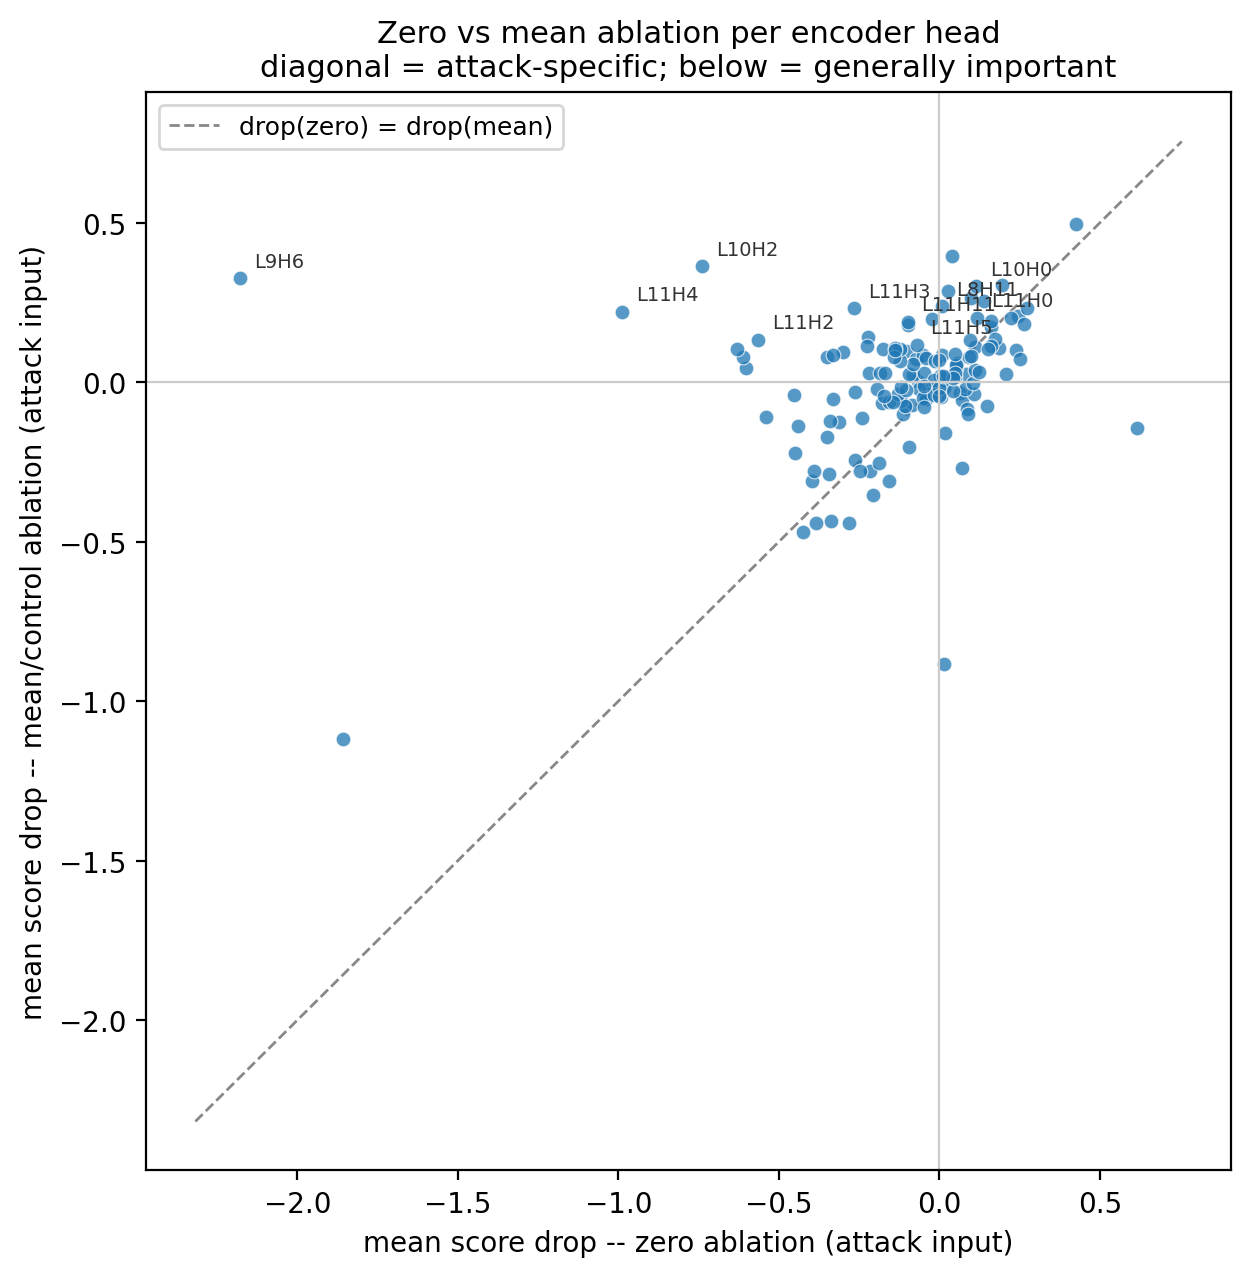
\includegraphics[width=0.65\textwidth]{outputs/plots/exp11_zero_vs_mean_ablation_scatter.png}
  \caption{Zero vs.\ mean/control ablation score drop, per head (canonical attack).
  Points far below the diagonal (\texttt{L9H6}: drop(zero)$=-2.18$ vs.\
  drop(mean)$=+0.33$) show zero ablation manufacturing large apparent importance that
  mean/control ablation does not corroborate.}
  \label{fig:scatter}
\end{figure}

Exactly Experiment 3's decoder finding, unchanged on the encoder: zero ablation
(replacing a head's contribution with the zero vector) produces score drops many times
larger than mean/control ablation for the same head (\texttt{L9H6}: $-2.18$ vs.\ the
mean-ablation-consistent \texttt{combined\_effect} of $0.087$) — zeroing pushes the model
far outside its normal operating distribution rather than isolating the head's
attack-specific contribution. This confirms mean/control ablation (used as the primary
metric everywhere above) was the right default, not just an inherited convention.

\subsection{The early-layer instability, again}
\label{sec:earlylayerinstability}

\begin{figure}[H]
  \centering
  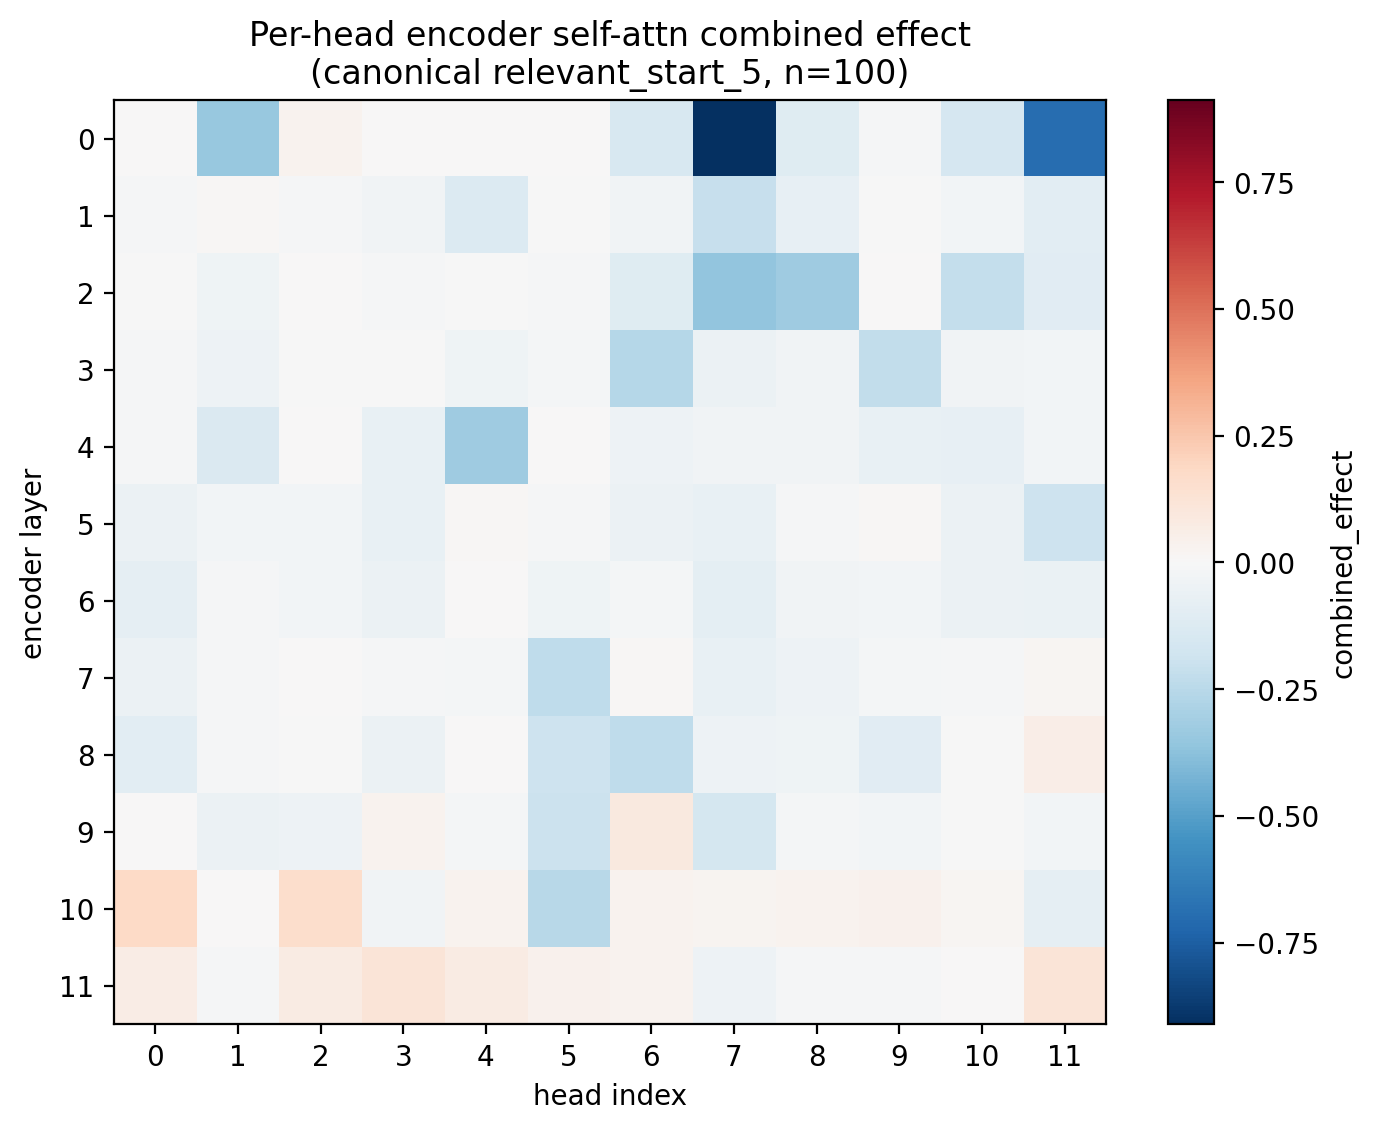
\includegraphics[width=0.7\textwidth]{outputs/plots/exp11_head_heatmap_canonical.png}
  \caption{Full-range heatmap, all 12 layers. \texttt{L0H7} ($\comb=-0.91$, driven almost
  entirely by $\rev=-0.91$ with $\fwd\approx0$) and \texttt{L0H11} ($-0.70$) dominate the
  colour scale, matching Experiment 6's documented early-layer instability: a
  single-head patch leaves the residual stream internally inconsistent for 11 more
  layers to process, amplify, or invert, before the score is read out.}
  \label{fig:fullheatmap}
\end{figure}

This is the third experiment in this project (after Experiment 6's position-restricted
patching) to independently reproduce the same qualitative pattern: partial-coverage
patches at early encoder layers produce large, sometimes sign-flipped effects that have
nothing to do with the patched region's true importance — a structural property of
patching a small subset of the network with many remaining layers to process the
inconsistency, not a per-experiment quirk.

% =====================================================================
\section{Overall Interpretation and Discussion}
% =====================================================================

\begin{enumerate}
  \item \textbf{The encoder-side effect is head-sparse, closing the gap Experiment 3
  left open.} 18 of 144 head-slots matter on the canonical attack, and the top 5 are
  robust on 100+ of 105 attacks — a reviewer can no longer ask "why decompose the
  decoder but not the encoder?"; the answer is now the same for both: sparse, not
  uniform, and the identity of the important heads is now a ranked, cross-validated
  list (Table~\ref{tab:top10}) rather than an assumption.
  \item \textbf{The additivity prediction failing is itself informative.}
  Super-additivity ($1.76\times$, not the predicted $\sim 0.44\times$ sub-additive
  pattern) means this project's template-position finding does not generalise
  automatically to heads — different intervention granularities can have qualitatively
  different composition behaviour, and future combination-search work (Phase 4) needs to
  measure combined effects directly rather than assume either additive or sub-additive
  composition from single-unit numbers.
  \item \textbf{The layer-9 attention anomaly is real but narrow; it does not explain
  layers 10--11.} Only 2 of 12 layer-9 heads are simultaneously high-mass and causally
  important, and the pattern does not extend to layers 10--11 at all, where 4 of the 5
  top-effect heads have unremarkable attention mass. Raw attention explains a real but
  small fraction of this experiment's localised effect — most of it is invisible to a
  purely descriptive, attention-based analysis, and would have been missed entirely
  without the causal patching this experiment ran.
  \item \textbf{The attack-token-as-hub story is real but not unifying.} The strongest
  individual head (\texttt{L9H6}) is a counterexample to its own aggregate trend — it is
  causally critical without the attack token attending unusually to the query. At least
  two distinct sub-mechanisms produce the same layer-9--11 causal signature; a single
  "attack token reads query, decoder cross-attends to it" story is not sufficient on its
  own.
  \item \textbf{Zero ablation is not a reliable importance measure on the encoder
  either.} Confirms Experiment 3's decoder finding is a property of ablation methodology,
  not something specific to the decoder's single-step scoring.
\end{enumerate}

% =====================================================================
\section{Limitations and Threats to Validity}
% =====================================================================

\begin{itemize}
  \item \textbf{Whole-sequence, not per-position.} Step 1/2 patch a head at every
  position at once; a joint head$\times$position sweep (144 heads $\times$ ~150
  positions) was explicitly out of scope this pass.
  \item \textbf{Flagging uses two different definitions.} Steps 1/4/5 flag
  $(layer, head)$ slots from the canonical attack ($n{=}100$); Step 2/3 flags $head\_idx$
  (pooled over layers 9--11) from the full 105-attack sweep. Both are reported; see
  \texttt{DECISIONS.md} item 7.
  \item \textbf{Step 4/5 recompute attention fresh.} No per-head attention tensor from
  Experiment 6 survived to disk (verified directly), so Steps 4/5 run their own forward
  passes on the same example set rather than re-slicing saved data.
  \item \textbf{Single model/dataset.} Results are for monoT5-base on DL19, matching
  every prior experiment in this project.
\end{itemize}

% =====================================================================
\section{Reproducibility}
% =====================================================================

From \texttt{11\_monot5\_encoder\_head\_patching/}, with the \texttt{advseq2seq} conda
environment and Experiments 1 and 6's outputs present as sibling directories:

\begin{lstlisting}
pytest tests/                              # correctness checks (tiny random T5, CPU)
bash bash/run_encoder_head_patching.sh     # full pipeline (resume-safe)
\end{lstlisting}

\noindent On this run: SLURM job on 1$\times$ L40 GPU, $\approx$20~minutes wall-clock for
the full pipeline; outputs under \texttt{outputs/\{canonical,sweep,layer9\_crossref,
hub\_analysis\}/}, \texttt{outputs/plots/}, and the written per-step verdict in
\texttt{outputs/SUMMARY.md}.

% =====================================================================
\section*{Appendix: Glossary of Key Quantities}
\addcontentsline{toc}{section}{Appendix: Glossary of Key Quantities}
% =====================================================================

\begin{description}[leftmargin=1.6em,style=nextline]
  \item[head-slot] one (encoder layer, head index) pair; 144 total.
  \item[$\fwd$ / $\rev$ / $\comb$] forward/reverse/combined patching effect, identical
  formulas to Experiment 1, applied per head-slot instead of per layer-component.
  \item[zero / mean ablation] head contribution set to zero, or replaced by the
  padded-control (Type B) activation for that head. Mean is primary.
  \item[flagged head] combined\_effect $> 0.02$ (project-wide threshold, from
  Experiment 6's template-position classification).
  \item[normalized\_mass$(A\to B)$] attention mass from region $A$ to region $B$,
  normalised by $B$'s share of total sequence length. $>1$ means more attention than a
  uniform baseline predicts.
\end{description}

\end{document}
